\chapter{Social Engineering}\label{ch:SocialEngineering}



\section{Was ist Social Engineering?}

Auch zum Thema Social Engineering lassen sich mehrere Definitionen finden, die in vielen Punkten übereinstimmen aber sich auch in wesentlichen Punkten unterscheiden. 

>>Beim Social Engineering werden menschliche Eigenschaften wie Hilfsbereitschaft, Vertrauen, Angst oder Respekt vor Autorität ausgenutzt, um Personen geschickt zu manipulieren. Cyber-Kriminelle verleiten das Opfer auf diese Weise beispielsweise dazu, vertrauliche Informationen preiszugeben, Sicherheitsfunktionen auszuhebeln, Überweisungen zu tätigen oder Schadsoftware auf dem privaten Gerät oder einem Computer im Firmennetzwerk zu installieren.<<\cite{bsi}

>>Social Engineering benutzt Techniken der Beeinflussung und Überredungskunst zur Manipulation oder zur Vortäuschung falscher Tatsachen, über die sich ein Social Engineer eine gefälschte Identität aneignet. Damit kann der Social Engineer andere zu seinem Vorteil ausbeuten, um mit oder ohne Verwendung von technischen Hilfsmitteln an Informationen zu gelangen.<<\cite{mitn}

Diese Definitionen betrachten Social Engineering durchweg als negativ, da es zum Schaden anderer und zum eigenen Vorteil eingesetzt wird. In anderen Quellen werden jedoch auch Definitionen dargestellt die aufzeigen dass Sozial Engineering auch zum Vorteil der Zielperson genutzt werden kann.

>>Social Engineering [...] nennt man zwischenmenschliche Beeinflussungen mit dem Ziel, bei Personen bestimmte Verhaltensweisen hervorzurufen, sie zum Beispiel zur Preisgabe von vertraulichen Informationen, zum Kauf eines Produktes oder zur Freigabe von Finanzmitteln zu bewegen.

Gleichzeitig steht Social Engineering für eine Praxis der politischen und gesellschaftlichen Steuerung bzw. Beeinflussung von Gesellschaften mittels Kommunikation und kann sowohl als positiv als auch als negativ wahrgenommene Ergebnisse erzielen. Die stark negative Begriffsvariante dominiert jedoch aktuell das Begriffsbild [...]<<\cite{wiki}

>>Akt der Manipulation einer Person, eine Handlung auszuführen, die vielleicht im besten Interesse der >>Zielperson<< liegt - oder auch nicht.<<\cite{Hadn1}


Die verschiedenen Definitionen stimmen darin überein, dass Social Engineering die Manipulation und/oder Beeinflussung von Personen umfasst, mit dem Ziel, diese zu bestimmten Handlungen zu veranlassen.

Social Engineering wird von verschiedenen Akteuren, darunter Einzelpersonen und Institutionen, zu unterschiedlichen Zwecken eingesetzt.

>>Ärzte Psychologen und Therapeuten nutzen beispielsweise oft Elemente des Social Engineering um ihre Patienten zu bestimmten Handlungen zu manipulieren. Trickbetrüger hingegen nutzen Elemente des Social Engineering um ihre Zielperson zu Aktivitäten zu bringen die zu einem Verlust führen.<< \cite{Hadn1}

Methoden des Social Engineering finden ebenfalls Anwendung im Vertrieb, wo Verkäufer Kunden Produkte aufdrängen, die diese möglicherweise gar nicht benötigen. Ähnliche Techniken werden auch von Personalrekrutierern, Regierungen und Spionen genutzt, jeweils angepasst an ihre spezifischen Ziele und Kontexte. (Vgl. \cite{werSE})
Auch verärgerte Angestellte können Methoden des Social Engineering nutzen um dem eigenen Unternehmen zu schaden. (Vgl. \cite{Hadn2})
Ebenso wie unterschiedliche Akteure die Social Engineering betreiben sind auch die Motivationen für einen Angriff unterschiedlich. Die einen tun es aus Spaß, für das Machtgefüh oder Rache während es für andere um Politik, Spionage oder Industriespionage geht. (vgl. \cite{Motivation})

\section{Geschichte des Social Engineering}

Social Engineering ist ein Phänomen, das es bereits seit Anbeginn der Menschheit gibt, auch wenn es nicht immer unter diesem Begriff bekannt war. Schon kleine Kinder weinen absichtlich, um bei ihren Eltern ihren Willen durchzusetzen, oder nutzen nonverbale Kommunikation, um Dinge zu erreichen, die sie sonst nicht bekämen. Dieses Verhalten zeigt, dass die Manipulation anderer durch gezielte Handlungen tief in der menschlichen Natur verankert ist. (vgl. \cite{SEinNaturdesMenschverankert})

Ein prominentes frühes Beispiel für Social Engineering ist das trojanische Pferd, das als der erste aufgezeichnete Social Engineering Angriff gilt. Diese Episode wurde in Homers "Odyssee" niedergeschrieben. Im Jahr 1184 v. Chr. nutzten die Griechen eine Täuschung, um in Troja einzudringen. Sie bauten ein Holzpferd als Geschenk und täuschten ihren Rückzug vor. Nach der Verkündung dass das Pferd ein Weihegenschenk an die Göttin Athene sei und Unglück bringt sollte es zerstört werden. Außerdem wurde es so groß gebaut damit es nicht in Stadt gebracht werden kann da die Stadt sonst unter dem Schutz der Athene stünde. Die Trojaner holten aufgrund dieser Manipulation das Pferd in die Stadt. Als die Trojaner schliefen, kletterten griechische Soldaten aus dem Holzpferd und öffneten die Tore von innen. (vgl. \cite{troja}).

Zum ersten Mal erwähnt wurde der Begriff Social Engineer in einem Zeitungsartikel der New York Times von 1887. T. Burnett Baldwin wurde darin als Social Engineer bezeichnet, der sichergestellt hat, dass seine Mitarbeiter das Karnevallsprogramm bis ins kleinste Detail ausführten.(vgl. \cite{nytimes1}) Im Jahr 1899 prägte William Tolman den Begriff "Social Engineering" und bezeichnete es als eine der neuesten Professionen. Tolman beschrieb in einem Artikel, wie eine Organisation ein leeres Grundstück in einen Erholungsbereich für die Familien der Mitarbeiter umwandelte, was zu einer verbesserten Beziehung zwischen den Mitarbeitern und dem Arbeitgeber führte.(vgl. \cite{nytimes2}) Dies zeigt, dass Social Engineering darauf zielt, auf eine Personengruppe Einfluss zu nehmen, um ihre Verbindung zu einer bestimmten Organisation zu intensivieren. (vgl. \cite{hist1}).

In der Geschichte der Menschheit finden sich jedoch immer wieder Beispiele dafür, wie Methoden des Social Engineering eingesetzt wurden, um Menschen in eine bestimmte Richtung zu lenken. Durch religiöse Regeln wurden ganze Kulturen geformt, die nach bestimmten Normen und ethischen Grundsätzen handeln, da sie sich davon Vorteile im Jenseits erhoffen. Ein prominentes Beispiel dafür ist das Kastensystem in Indien, das tief in religiösen Überzeugungen und sozialen Strukturen verwurzelt ist und seit Jahrtausenden das Verhalten und die Interaktionen der Menschen bestimmt (vgl. \cite{hindu}).

Ein weiteres Beispiel ist die Verwendung von Propaganda durch politische Regime, um die öffentliche Meinung zu beeinflussen und die Macht zu festigen. Während des Zweiten Weltkriegs nutzten verschiedene Länder intensiv Propaganda, um die Moral zu stärken und die Bevölkerung hinter den Kriegsanstrengungen zu vereinen (vgl. \cite{hisofpropaganda}). Diese gezielte Beeinflussung der Massen zeigt, wie tiefgreifend und wirkungsvoll Social Engineering sein kann.

In modernen Zeiten hat sich Social Engineering weiterentwickelt und ist zu einem zentralen Thema im Bereich der Informationssicherheit geworden. Cyberkriminelle nutzen psychologische Manipulationstechniken, um Menschen dazu zu bringen, vertrauliche Informationen preiszugeben oder schädliche Software herunterzuladen. Dieses Phänomen zeigt, dass Social Engineering nicht nur ein historisches, sondern auch ein aktuelles und sich ständig weiterentwickelndes Thema ist (vgl. \cite{mitn1}).


\section{Grundformen des Sozial Engineering}

Es existieren diverse Methoden, wie Social Engineers Zugang zu ihren Zielobjekten erlangen, wobei sich die Vorgehensweisen in technische, physische und über soziale Medien vermittelte Ansätze unterteilen lassen.

Technisches Social Engineering umfasst Angriffe, die mithilfe von technischen Geräten wie Computern, Handys oder Telefonen durchgeführt werden. Hierbei werden oft komplexe technische Hilfsmittel eingesetzt, um Sicherheitsmaßnahmen zu umgehen und Zugang zu vertraulichen Informationen zu erlangen.

Physisches Social Engineering bezieht sich auf Situationen, in denen der Angreifer persönlich in Erscheinung tritt, um sein Ziel zu erreichen. Dies kann beispielsweise durch das Eindringen in gesicherte Gebäude unter falscher Identität oder durch direkte Interaktion mit dem Ziel unter einem Vorwand geschehen.

Bei Angriffen über soziale Medien nutzen Social Engineers ebenfalls technische Hilfsmittel, um zunächst Kontakt zur Zielperson aufzubauen. Die eigentliche Manipulation erfolgt jedoch durch persönliche Kommunikation über Plattformen wie Chats, Messenger-Dienste oder andere soziale Netzwerke. Hierbei wird oft eine Kombination aus technischem Know-how und psychologischen Fähigkeiten eingesetzt, um die Zielperson subtil zu beeinflussen.

Diese Kategorisierung verdeutlicht, wie vielseitig und angepasst Social Engineering-Methoden sein können, je nach Ziel und Kontext des Angriffs. (Vgl. \cite{SEtechPhysSoc})

\begin{figure}[h]
    \centering
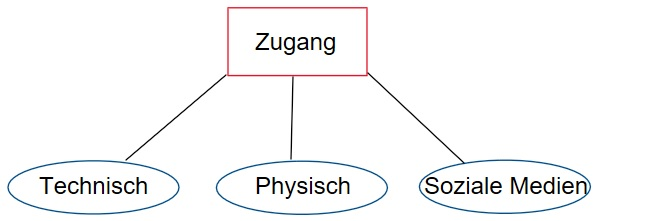
\includegraphics[width = 10cm]{figures/Zugang.jpg}
\caption{verschiedene Zugangsarten}
(eigene Darstellung)
\label{fig:verschiedene Zugangsarten}
\end{figure}

Social Engineering in seiner schädlichen Ausprägung lässt sich typischerweise in drei Hauptkategorien einteilen: Phishing, Elizitieren per Telefon und Identitätsbetrug (vgl. \cite{GrundformenDesSE})

\subsection{Phishing}

Phishing, ein Begriff, der sich aus den Worten "Passwort" und "Fishing" zusammensetzt, ist die am häufigsten auftretende Form des Social Engineering wie Abbildung \ref{fig:CrimeVergleich} zeigt.(vgl. \cite{bsi1})

\begin{figure}[h]
    \centering
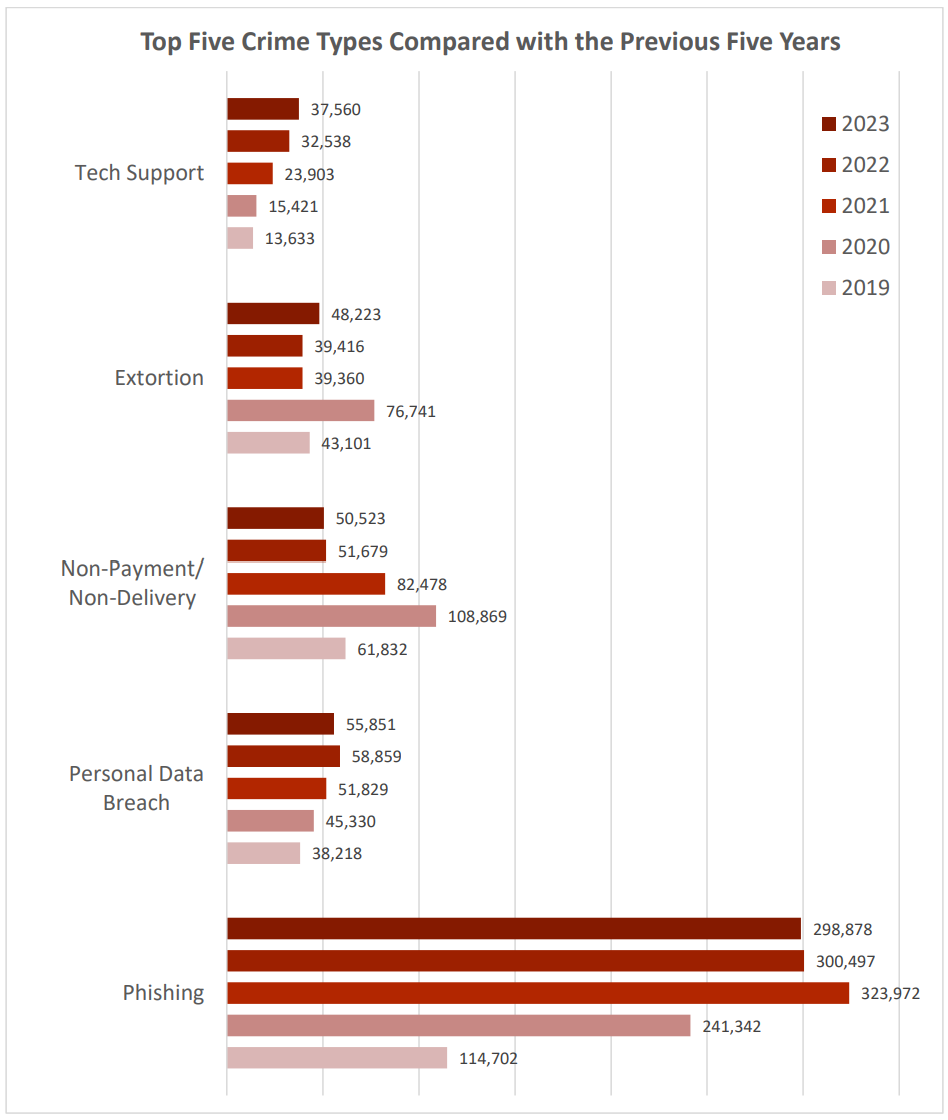
\includegraphics[width = 12cm]{figures/FBICrimeVergleich.png}
\caption{Die fünf häufigsten Kriminalitätsarten im Vergleich zu den letzten fünf Jahren}
\cite{fbi}
\label{fig:CrimeVergleich}
\end{figure}

Phishing gehört zum technischen Social Engineering. Bei dieser Methode senden Angreifer massenhaft E-Mails, die gezielt Emotionen wie Angst und Neugier oder das Konzept der Autorität ausnutzen. Diese E-Mails enthalten schädliche Dateien, Links oder Anweisungen. Das Anklicken, Öffnen oder Befolgen dieser Inhalte kann zu Datenverlust, Sicherheitsverletzungen oder anderen nachteiligen Konsequenzen für die Zielperson führen(Vgl. \cite{phishing}) Abbildung \ref{fig:PhishingPayPal} zeigt eine solche E-mail.


\begin{figure}[h]
    \centering
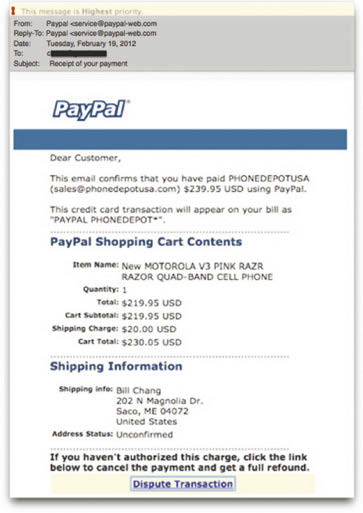
\includegraphics[width = 7cm]{figures/ChristopherHadn_2014_Kapitel2WasIstSocialE_SocialEngineeringEntt.jpg}
\caption{gefälschte E-Mail von PayPal}
\cite{GrundformenDesSE}
\label{fig:PhishingPayPal}
\end{figure}

Die Befürchtung, dass das eigene Konto kompromittiert und Geld gestohlen wurde, kann ausreichen, um einen Menschen dazu zu bewegen, auf einen Link zu klicken und sich schnell ins Konto einzuloggen, um die Situation zu überprüfen. Genau diese Reaktion intendiert der Angreifer. Häufig werden die Zugangsdaten dann von einer gefälschten Webseite oder durch einen manipulierten Login-Prozess mittels kleiner Skripte abgefangen. Sobald der Angreifer diese Daten in seinem Besitz hat, nutzt er sie, um sich einzuloggen und genau jene Handlung auszuführen, vor der das Opfer Angst hatte: das Geld wird gestohlen. (Vgl. \cite{phishing}) Da es sich hierbei um Massen-E-Mails handelt ist die Anrede immer unpersönlich. \\
Wenn solche Angriffe durch persönlich angepasste E-Mails ausgeführt werden, die bereits detaillierte Informationen, wie Vorlieben oder Abneigungen, des Empfängers enthalten, bezeichnet man dies als >>Spear-Phishing<<. Dieser Begriff leitet sich vom Speer ab, der als Symbol für die gezielte Ausrichtung auf ein spezifisches Ziel steht. (Vgl. \cite{spear},\cite{phishing})\\
Eine Spezialform des Spear-Phishing ist das >>Whaling<<, auch bekannt als >>CEO-Fraud<< oder >>Business E-Mail Compromise (BEC)<<. Whaling leitet sich von Wal ab und umschreibt das Spear-Phishing auf ein hochrangiges Individuum, wie z.B. den CEO einer Firma. >>Allein im Jahr 2023 erhielt das IC3 des FBI 21.489 BEC-Beschwerden, wobei die angepassten Verluste über 2,9 Milliarden Dollar betrugen.<<\cite[frei übersetzt]{fbi}


\subsection{Elizitieren per Telefon}

Das \glqq Elizitieren\grqq{} am Telefon ist die zweithäufigste Methode des Social Engineering.\cite{eliAmTel} \glqq In Schulungsunterlagen definiert die National Security Agency der USA Elizitieren als \glq subtile Extraktion von Informationen während einer offenbar normalen und harmlosen Unterhaltung\grq\grqq{}.\cite{elizitieren}

Beim Elizitieren per Telefon kontaktiert der Angreifer die Zielperson telefonisch und stellt unauffällige Fragen, um relevante aber bedeutungslos wirkende Informationen zu sammeln. Diese Informationen nutzt er häufig, um bei der nächsten Zielperson vertrauenswürdig zu erscheinen und so Zugang zu sensibleren Daten zu erhalten.

Typischerweise verwendet der Angreifer einen \glqq Pretext\grqq{}, indem er vorgibt, eine Person mit berechtigtem Interesse an den Informationen zu sein. (Vgl. \cite{eliz}) \glqq Mit Pretexting bezeichnet man die Schaffung eines erfundenen Szenarios, um die Zielperson als Opfer dazu zu überreden, Informationen herauszurücken oder eine Aktion auszuführen.\grqq{} \cite{pretext} Dies wird durch \glqq Spoofing\grqq{}unterstützt, wobei der Zielperson eine falsche Telefonnummer angezeigt wird, um den Eindruck zu erwecken, der Anruf stamme von einer vertrauenswürdigen Quelle(Vgl. \cite{spoofing})

Die Effektivität des Elizitierens beruht auf der psychologischen Manipulation der Zielperson. Durch geschicktes Fragen und das Erzeugen eines Gefühls von Vertraulichkeit und Dringlichkeit gelingt es dem Angreifer, die Zielperson dazu zu bringen, Informationen preiszugeben, die sie unter normalen Umständen nicht teilen würde. Dies wird oft durch nonverbale Kommunikation wie Lächeln, Tonfall oder Sprechgeschwindigkeit unterstützt. Diese Technik erfordert sowohl Geduld als auch ein gutes Verständnis menschlicher Verhaltensweisen, um erfolgreich zu sein. (Vgl. \cite{elizitieren1})

Auch die Polizei warnt vermehrt vor Betrügern, die sich am Telefon als Polizisten ausgeben und mit gefälschter Telefonnummer warnen das ein Einbruch ins Anwesen des Opfers bevorsteht. Sie fordern das Opfer auf Barvermögen und Wertgegenstände zur Sicherheitsverwahrung an falsche Kollegen zu übergeben. Außerdem soll das Opfer mit niemanden darüber sprechen um angebliche Ermittlungen nicht zu gefährden. Siehe Abbildung \ref{fig:Polizei} (Vgl. \cite{polizeibeamte})   

\begin{figure}[h]
    \centering
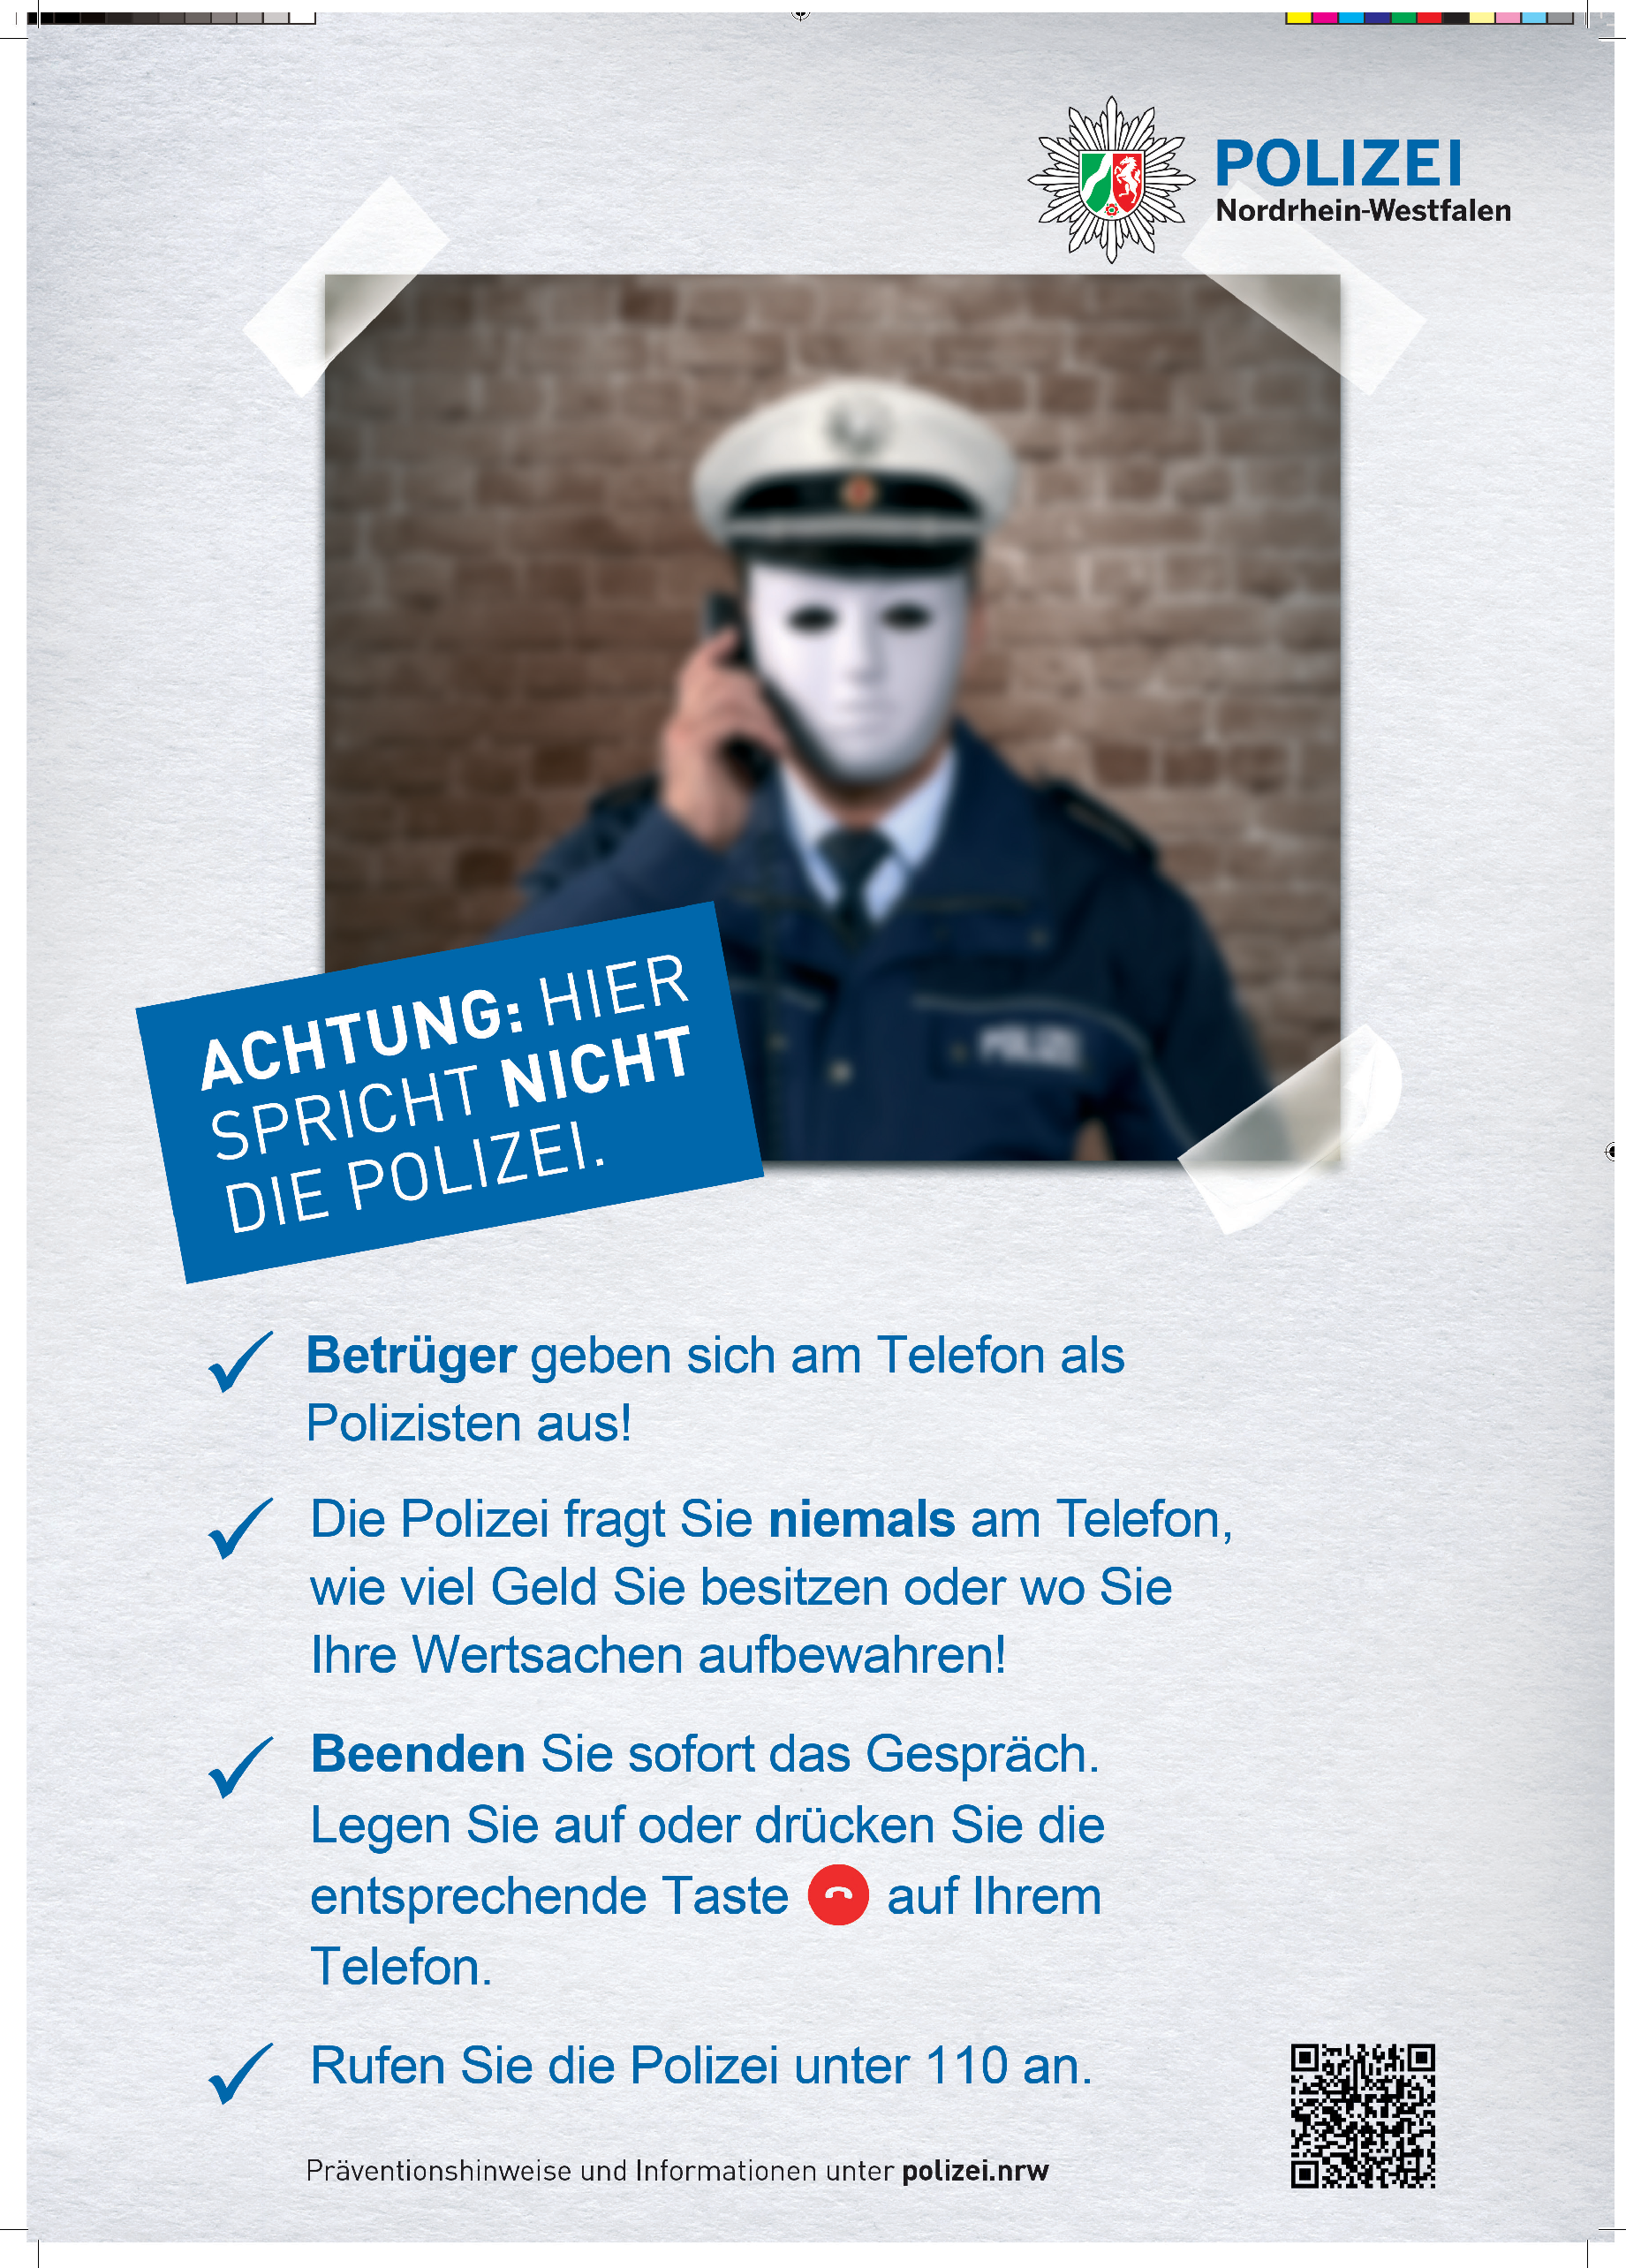
\includegraphics[width = 5cm]{figures/LKA-Dokument-Poster-Falsche-Polizei NEU.pdf}
\caption{Poster der Polizei Nordrhein-Westfalen}
\cite{polizeibeamte}
\label{fig:Polizei}
\end{figure}

\subsection{Identitätsbetrug}

Beim Identitätsbetrug übernehmen die Angreifer eine fremde Identität, um die Zielperson zu unvorteilhaften Handlungen zu bewegen. Auch hier spielen Elizitieren und Pretexting eine wichtige Rolle. Im Gegensatz zu Phishing und telefonischem Elizitieren ist Identitätsbetrug eine physische Methode des Social Engineering. Daher kommt der nonverbalen Kommunikation eine besondere Bedeutung zu. Abhängig vom gewählten Pretext des Angreifers ist es entscheidend, die nonverbalen Signale der Zielperson richtig zu interpretieren und gleichzeitig selbst die passenden nonverbalen Zeichen auszusenden. (Vgl. \cite{Identitätsbetrug})

Eine Beliebte Methode des Identitätsbetrugs ist \glqq Tailgating\grqq{}. Hierbei folgt der Angreifer befugten Personen in einen Bereich zu dem er sonst keinen Zutritt hätte indem er sich als jemand ausgibt, der berechtigt ist einzutreten. Indem er sich beispielsweise als Mitarbeiter ausgibt und im schwächer gesicherten Raucherberich aufhält um mit den Mitarbeitern anschließend das Gebäude zu betreten. Oft reicht es auch einen großen Karton zu tragen während man auf eine gesicherte Tür zuläuft, um von einem hilfsbereiten Mitarbeiter die Tür aufgehalten zu bekommen. Ein weiterer beliebter Trick ist es eine Kennkarte optisch zu kopieren. Nach mehreren Fehlversuchen besteht eine hohe Chance eingelassen zu werden. Diese Taktiken funktionieren besser, wenn sich der Angreifer gut vorbereitet hat und Verhaltensweisen, Körpersprache, Dialekte und Kleidungsstil der Angestellten erforscht und eingeübt hat. Auch hier hilft es im Vorfeld zu Elizitieren um an die notwendigen Informationen zu kommen. (Vgl. \cite{Identitätsbetrug})

Bei einem Identitätsbetrug wie in dem Fall der falschen Polizisten, benutzen die Angreifer falsche Uniformen um sich als Polizisten auszugeben. Hier müssen die Täter versuchen sowohl Vertrauen als auch Autorität auszustrahlen um die Opfer nicht misstrauisch zu machen. 

%Hauptmann von Köpenick
\section{weitere Angriffsvektoren}

\subsection{Dumpster diving}
\subsection{Watering Hole}
\subsection{Ködern}
\subsection{Honigtopf}
\subsection{USB Drop}



\section{Psychologische Prinzipien hinter Social Engineering}

% Framing
% Rapport
% Microexpressionen
% Manipulation

\subsection{6 Prinzipien der Beeinflussung}
Es gibt viele unterschiedliche Taktiken die Social Engineere nutzen um ihre Zielperson zu überzeugen. Die meisten davon haben ihren Kern in einem von sechs grundlegenden psychologischen Prinzipien (vgl. \cite{PsychDesÜberzeugens}). Diese Prinzipien werden im folgenden kurz vorgestellt und erklärt wie ein Angreifer diese nutzt um seine Zielperson zu beeinflussen.  

\subsubsection{Reziprozität}

\glqq Nach Erkenntnissen von Soziologen und Anthropologen ist eine der verbreitetsten und grundlegensten Normen der menschlichen Kultur die Reziprotzitätsregel. Diese Regel besagt, dass Menschen versuchen sollen sich für das zu revanchieren, was sie von anderen bekommen.\grqq{} \cite{PsychDesÜberzeugensRezi} Diese Regel wurde Menschen bereits in Kindestagen beigebracht, zumeist mit der Redewendung \glqq Eine Hand wäscht die andere\grqq{}. Die Regel hat für eine Gesellschaft enorme Vorteile, indem sie den Ausbau des Handels, der Verteidigung und der gegenseitigen Hilfeleistung ermöglicht (vgl. \cite{rezi}). 

Ein Angreifer kann die Regel auszunutzen, indem er durch kleine Gefälligkeiten, Geschenke oder Zugeständnisse die Zielperson dazu bringen kann, zu tun was den Wünschen des Angreifers entspricht um nicht in dessen Schuld zu stehen (vgl. \cite{rezi}).


\subsubsection{Verpflichtung und Konsistenz}

Die meisten Menschen wollen konsequent erscheinen. Sie wollen in ihren Worten Überzeugungen und Taten konsistent sein da die Gesellschaft der Konsistenz einen hohen Wert beimisst und sie sich im Alltag gut bewährt. Eine Orientierung am Konsistenzprinzip hilft schnelle Entscheidungen zu treffen, ohne alle relevanten Informationen prüfen zu müssen, indem man im Einklang mit früheren Entscheidungen und festgelegten Standpunkten handelt.    

Der Angreifer versucht die Zielperson dazu zu bringen einen bestimmten Standpunkt zu beziehen. Die Zielperson spührt eine Verpflichtung konsequent zu sein und bei diesem Standpunkt zu bleiben. Wenn der Angreifer nun bittet Handlungen auszuführen die mit diesem Standpunkt im Einklang stehen, ist die Zielperson eher geneigt diesen Bitten oder Aufforderungen nachzugehen. Wenn Menschen sich öffentlich und aktiv auf einen Standpunkt festgelegt haben, dies mit Mühen verbunden war und durch innere Überzeugung geschah, ist die Verpflichtung noch größer (vgl.\cite{PsychDesÜberzeugensCom}). \glqq Die Konsistenz ist so stark, das Menschen gegen ihre eigenen Interessen verstossen, nur um nach außen hin als Konsistent zu gelten.\grqq{} \cite{ComundKon}

\subsubsection{Soziale Bewährtheit}

Das Prinzip der sozialen Bewährtheit besagt das Menschen dazu neigen ihre Entscheidungen wie sie handeln und was sie glauben danch auszurichten was andere Menschen in dieser Situation glauben oder machen. Das Verhalten der anderen Personen wird in diesem Moment als richtig angenommen. Wenn Personen unsicher sind, da eine mehrdeutige Situation vorliegt wird dieses Verhalten noch verstärkt. Auch die Festellung einer Ähnlichkeit zu anderen Personen verstärkt dieses Verhalten.

Ein Angreifer kan dieses Prinzip benutzen um die Zielperson zu einer Handlung zu ermutigen indem er sie in eine unsichere Situation bringt und darauf hinweist dass schon viele andere Personen genauso gehandelt haben. (vgl. \cite{PsychDesÜberzeugensSozBew})


\subsubsection{Sympathie}

\glqq Menschen sind eher bereit, sich von jemandem überzeugen zu lassen, den sie kennen und sympatisch finden.\grqq{} \cite{PsychDesÜberzeugensSym}
Der Mensch tendiert dazu, diejenigen zu mögen, die ihn mögen. \cite{sym}

Ebenso wie bei dem Prinzip der sozialen Bewährtheit, ist auch hier Ähnlichkeit ein Faktor der Einfluss darauf hat ob jemand eine andere Person sympatisch findet. Dabei ist es unabhängig davon ob sich dies in ähnlichen Meinungen Charaktereigenschaften oder Lebensweisen äußert. (vgl. \cite{sym1})
Ein weiterer Faktor bei der Entwicklung von Sympathie ist die körperliche Attraktivität. Einer Forschung zufolge werden Attraktiven Menschen unterbewusst automatisch positive Eigenschaften zugeschrieben (vgl. \cite{sym2}). Dies führt dazu, dass sie andere Personen leichter beeinflussen können. 
Wiederholte Kontakte unter positven Rahmenbedingungen mit einer Person, bestenfalls eine erfolgreiche Kooperation, sind ebenfalls gute Möglichkeiten um Sympathie zu erzeugen. (vgl. \cite{PsychDesÜberzeugensSymp})

Der Angreifer studiert seine Zielperson um sich ein möglichst genaues Bild von ihr zu machen. Sie passen ihren Kleidungsstiel an den der Zielperson an und achten darauf ein gepflegtes äuseres Erscheinungsbild abzugeben. Durch die Vortäuschung gleicher Interessen und gut plazierter Komplimente versuchen sie Sympathie zu erzeugen und so die Zielperson anfällig für ihre Wünsche und Forderungen zu machen. (vgl. \cite{PsychDesÜberzeugensSymp})


\subsubsection{Autorität}

Gehorsam gegenüber Autoritäten ist ein Prinzip das die Menschen schon seit Kindheitstagen prägt. Bereits Eltern bringen ihren Kindern bei das Gehorsam gegenüber den richtigen Autoritäten gut und Ungehorsam schlecht ist. Sie sollen ihren Eltern, Lehrern oder anderen Autoritäten gehorchen und sie nicht in Frage stellen da dies als respektlos gilt. Im Erwachsenenalter wird verlangt sich rechtlichen, militärischen und politischen Systemen unterzuordnen. Auch in der Bibel wird beschrieben, \glqq wie Ungehorsam gegenüber der höchsten Autorität dazu führte, dass Adam, Eva und der Rest der Menschheit des Paradieses verlustig gingen.\grqq{} \cite{PsychDesÜberzeugensBibel} 
In vielen Fällen ist es richtig auf die Anweisungen von Autoritäten zu befolgen da diese über Wissen Erfahrung und Macht verfügen. 
Oft reicht es auch schon den Anschein von Autorität zu erzeugen um automatischen Gehorsam zu erzeugen. Hierfür reichen oft schon die Insignien der Autorität, wie der richtige Titel, die passende Kleidung und Luxusartikel, wie Schmuk oder teure Fahrzeuge. (Vgl. \cite{PsychDesÜberzeugensAuto}) 

Der Angreifer benutzt die Insignien der Autorität, wie z.B. eine Uniform, Visitenkarte oder ein Luxusauto um der Zielperson zu suggerieren das er über Macht verfügt und Zielperson seinem Willen entsprechend handeln sollte. Hierbei ist auch die richtige Körpersprache, Stimme und Artikulation wichtig damit die Zielperson nicht misstrauisch wird und die Autorität hinterfragt. (Vgl. \cite{Auto})


\subsubsection{Knappheit}

Das Knappheitsprinzip besagt, \glqq dass Möglichkeiten uns umso wertvoller erscheinen, je weniger erreichbar sie sind\grqq{}\cite{PsychDesÜberzeugensKnapp1}. Das Verlangen einer Person kann durch zeitliche oder mengenmäßige Begrenzungen sowie durch Konkurrenzdruck gesteigert werden. \cite{PsychDesÜberzeugensKnapp}

Der Gedanke etwas zu verlieren motiviert die Menschen dabei stärker als der Gedanke etwas Gleichwertiges gewinnen zu können (vgl. \cite{Knapp}). Insbesondere in Situationen, die von Risiko und Unsicherheit geprägt sind, beeinflusst die Gefahr eines möglichen Verlustes die Entscheidungsprozesse erheblich (vgl. \cite{Knapp1},\cite{Knapp2}).

Wenn Wahlfreiheit beschnitten oder bedroht wird, steigt das Verlangen, diese Freiheiten sowie die damit verbundenen Produkte und Dienstleistungen zu behalten, erheblich an. Dies löst eine Gegenreaktion aus, die das Interesse an der Sache und die Bemühungen, sie zu erlangen, intensiviert. Dieser Effekt wird als \glqq Reaktanz\grqq{} bezeichnet. (Vgl. \cite{Knapp3}) 
Besonders augeprägt ist diese Reaktanz in der Trotzphase bei Kleinkindern und in der Pupertät bei Jugendlichen, da diese Lebensabschnitte durch ein aufkommendes Individualitätsgefühl gekennzeichnet sind. (Vgl. \cite{PsychDesÜberzeugensKnapp}) 

Das Knappheitsprinzip bezieht sich auch auf Informationen. Verschiedene Forschungsarbeiten haben gezeigt, dass Informationen die schwerer zu erhalten sind eine größere Überzeugskraft besitzen (vgl. \cite{ForschKnapp}, \cite{Knapp4}, \cite{ForschKnapp1}). Unterliegt die Infomation einer Zensur überzeugte sie sogar ohne dass die Information tatsächlich vorlag (vgl. \cite{Knapp4}). 

Beim Phishing wird häufig das Knappheitsprinzip eingesetzt. In den E-Mails wird von zeitlich begrenzten Angeboten oder Fristen gesprochen, nach deren Ablauf etwas Schlimmes passieren oder verloren gehen könnte. Ebenso werden exklusive Angebote, die auf geheimen Informationen basieren, verwendet, um die Opfer dazu zu verleiten, den Anweisungen zu folgen.

Angreifer können das Knappheitsprinzip auch nutzen um das Reziprotzitätprinzip zu verstärken.Indem sie Information teilen von den sie behaupten dass sie schwer zu bekommen waren, steigt der Wert dieser Gabe für die Zielperson die sich nun revanchieren möchte.
%\section{Beispiel eines erfolgreichen Social Engineering Angriffs}
